%!TEX root = ../paper.tex

%Ferdosi Sets 1
\begin{subfigure}{0.3\textwidth}
	\centering
	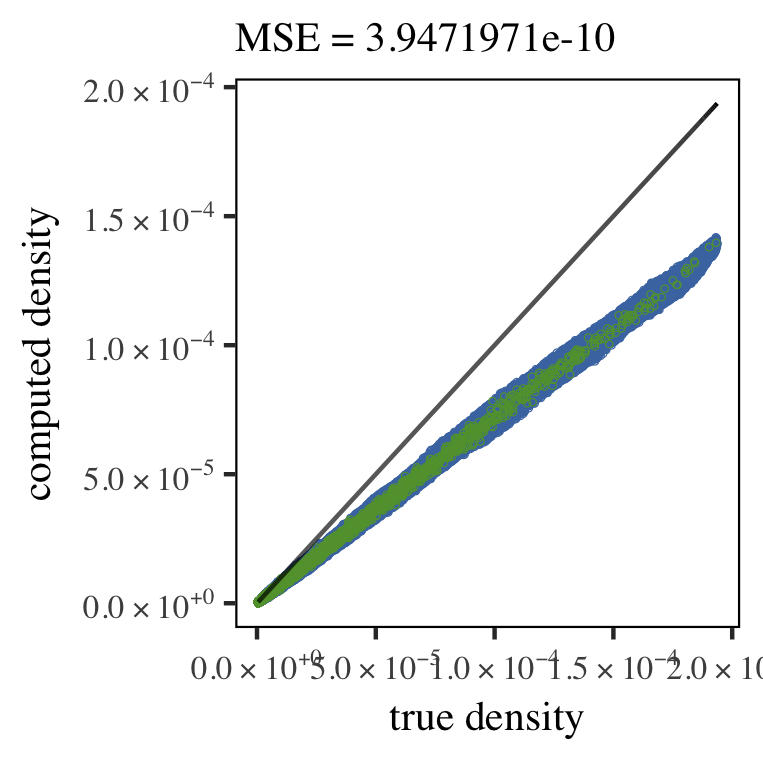
\includegraphics[keepaspectratio=true, width=\textwidth, height=0.23\textheight]{4/img/results_ferdosi_1_600000_parzen}
	\caption{Set \ferdosiOne}
	\label{fig:4:simulated:datasets:parzen:ferdosi1}
\end{subfigure}
% Ferdosi Set 2
\begin{subfigure}{0.3\textwidth}
	\centering
	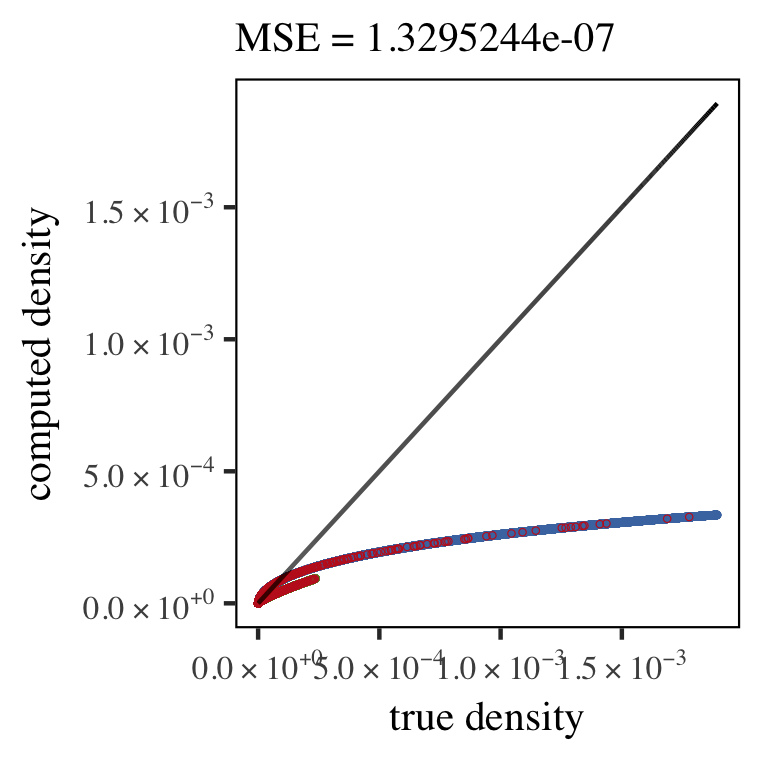
\includegraphics[keepaspectratio=true, width=\textwidth, height=0.23\textheight]{4/img/results_ferdosi_2_600000_parzen}
	\caption{Set \ferdosiTwo}
	\label{fig:4:simulated:datasets:parzen:ferdosi2}
\end{subfigure}	
% Ferdosi Set 3
\begin{subfigure}{0.3\textwidth}
	\centering
	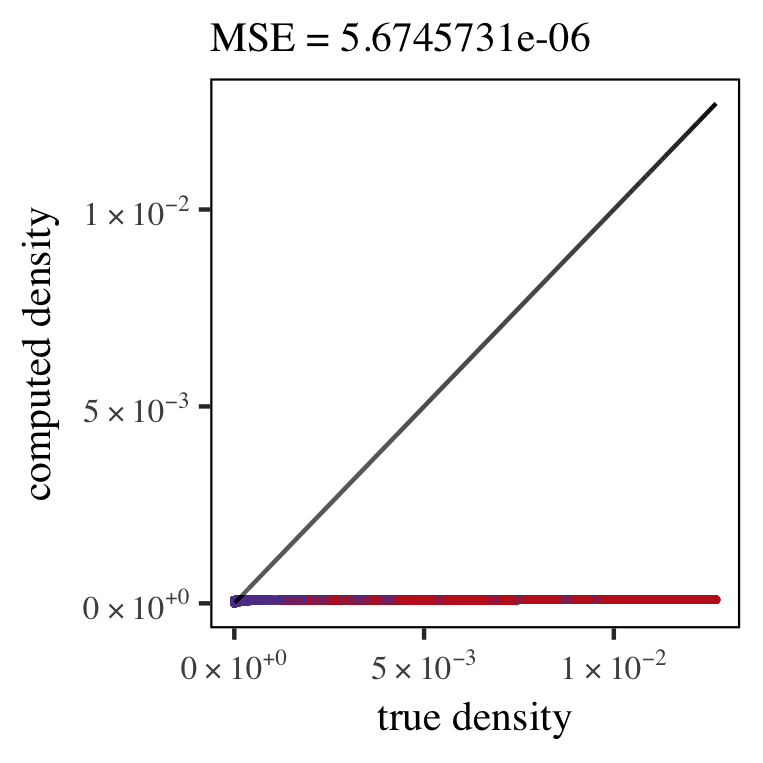
\includegraphics[keepaspectratio=true, width=\textwidth, height=0.23\textheight]{4/img/results_ferdosi_3_1200000_parzen}
	\caption{Set \ferdosiThree}
	\label{fig:4:simulated:datasets:parzen:ferdosi3}
\end{subfigure}	
% Baakman 1	
\begin{subfigure}{0.3\textwidth}
	\centering
	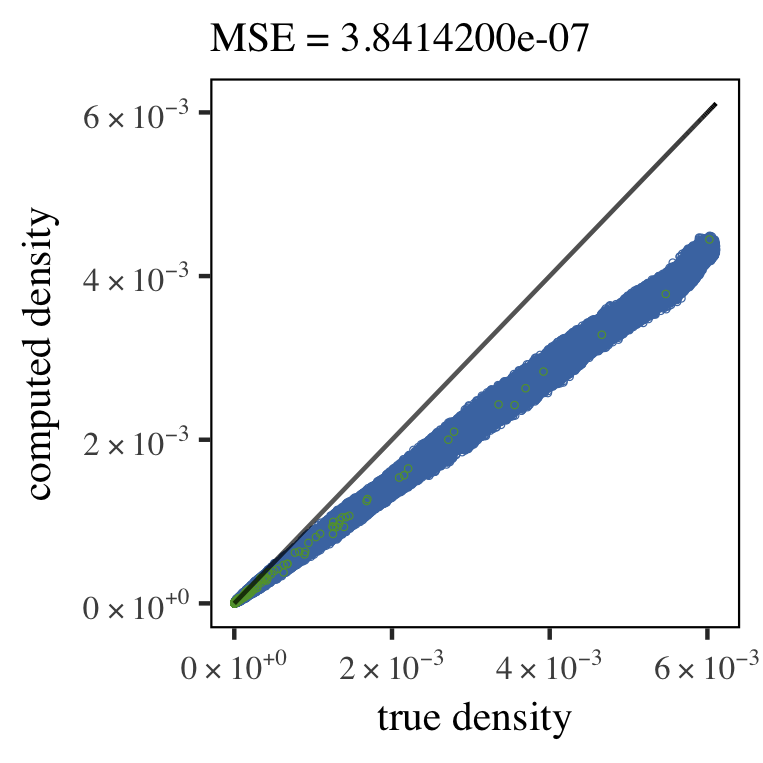
\includegraphics[keepaspectratio=true, width=\textwidth, height=0.23\textheight]{4/img/results_baakman_1_600000_parzen}
	\caption{Set \baakmanOne}
	\label{fig:4:simulated:datasets:parzen:baakman1}
\end{subfigure}
% Baakman 2
\begin{subfigure}{0.3\textwidth}
	\centering
	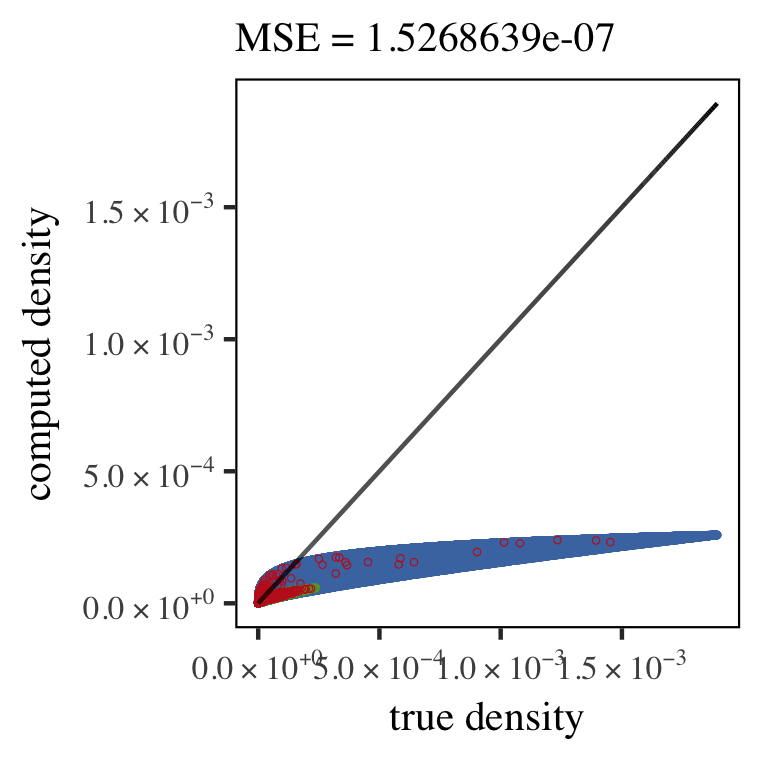
\includegraphics[keepaspectratio=true, width=\textwidth, height=0.23\textheight]{4/img/results_baakman_2_600000_parzen}
	\caption{Set \baakmanTwo}
	\label{fig:4:simulated:datasets:parzen:baakman2}
\end{subfigure}	
% Baakman 3
\begin{subfigure}{0.3\textwidth}
	\centering
	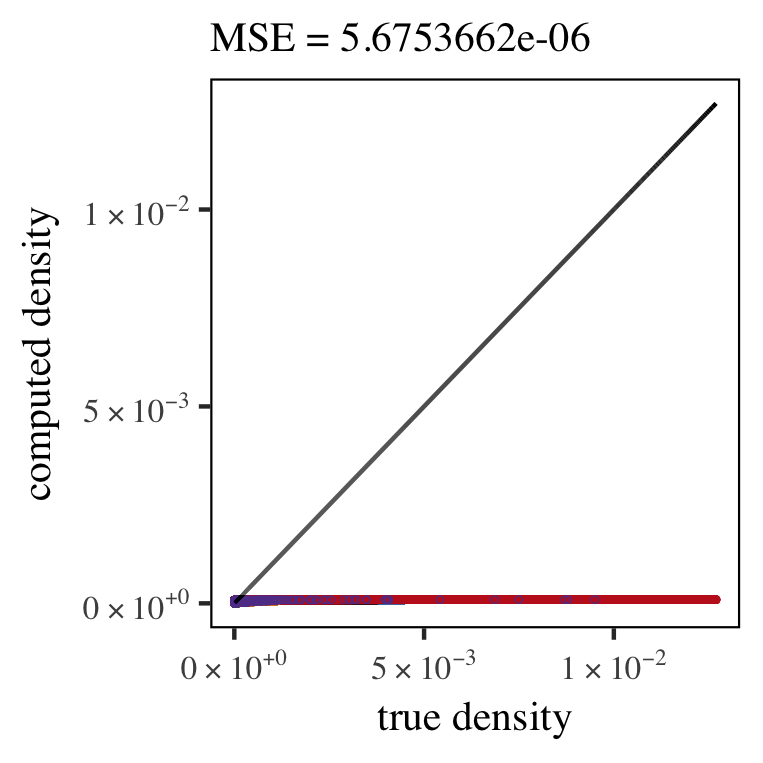
\includegraphics[keepaspectratio=true, width=\textwidth, height=0.23\textheight]{4/img/results_baakman_3_1200000_parzen}
	\caption{Set \baakmanThree}
	\label{fig:4:simulated:datasets:parzen:baakman3}
\end{subfigure}				
% Baakman 4
\begin{subfigure}{0.3\textwidth}
	\centering
	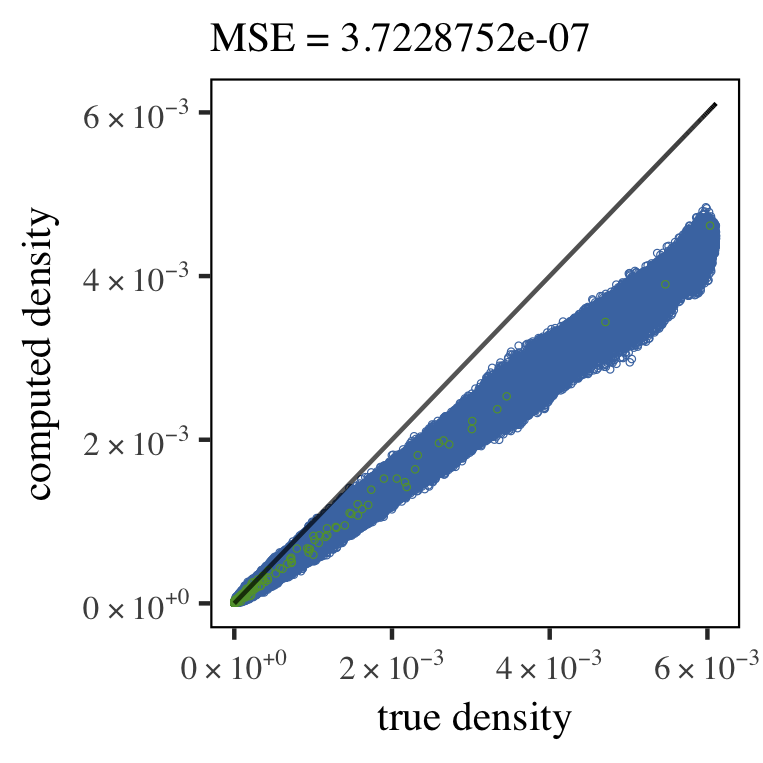
\includegraphics[keepaspectratio=true, width=\textwidth, height=0.23\textheight]{4/img/results_baakman_4_600000_parzen}
	\caption{Set \baakmanFour}
	\label{fig:4:simulated:datasets:parzen:baakman4}
\end{subfigure}	
% Baakman 5
\begin{subfigure}{0.3\textwidth}
	\centering
	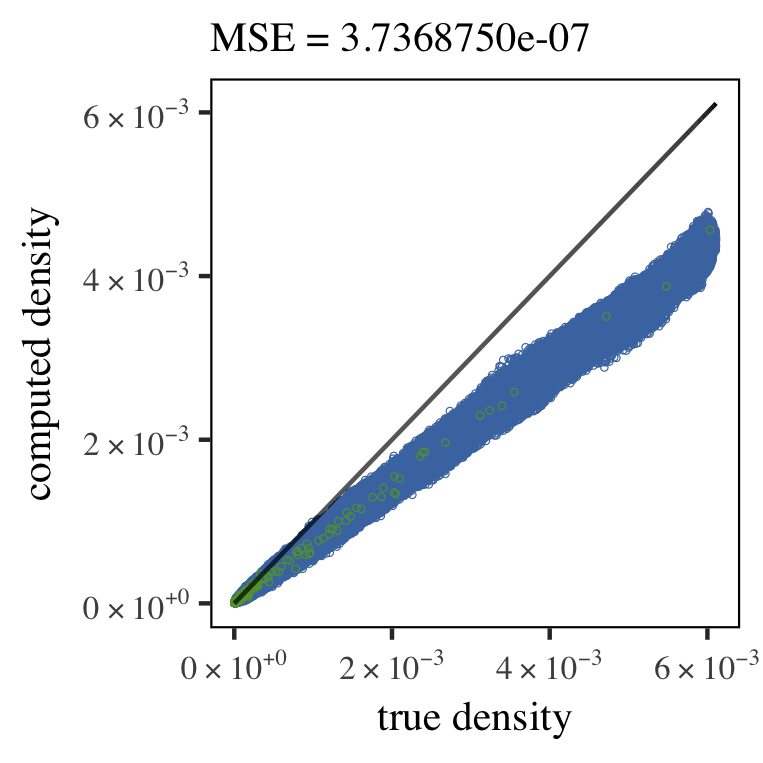
\includegraphics[keepaspectratio=true, width=\textwidth, height=0.23\textheight]{4/img/results_baakman_5_600000_parzen}
	\caption{Set \baakmanFive}
	\label{fig:4:simulated:datasets:parzen:baakman5}
\end{subfigure}		
% Ferdosi Set 4
\begin{subfigure}{0.3\textwidth}
	\centering
	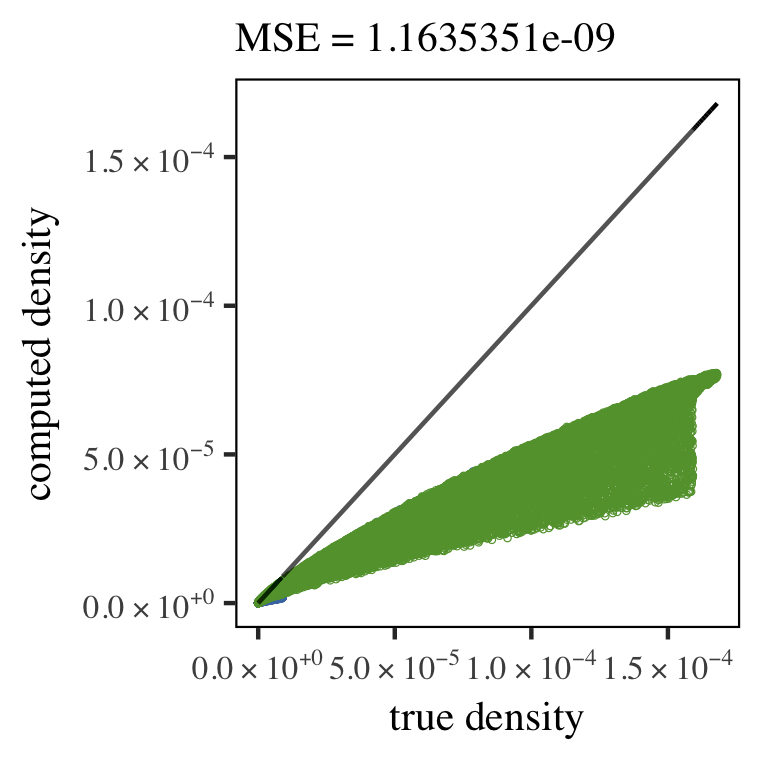
\includegraphics[keepaspectratio=true, width=\textwidth, height=0.23\textheight]{4/img/results_ferdosi_4_600000_parzen}
	\caption{Set \ferdosiFour}
	\label{fig:4:simulated:datasets:parzen:ferdosi4}
\end{subfigure}
% Ferdosi 5
\begin{subfigure}{0.3\textwidth}
	\centering
	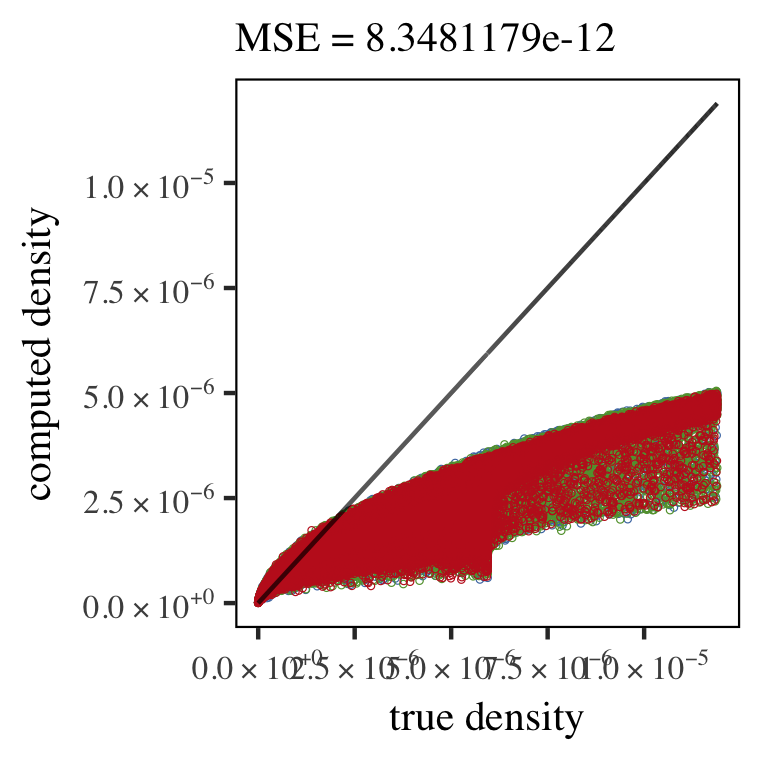
\includegraphics[keepaspectratio=true, width=\textwidth, height=0.23\textheight]{4/img/results_ferdosi_5_600000_parzen}
	\caption{Set \ferdosiFive}
	\label{fig:4:simulated:datasets:parzen:ferdosi5}
\end{subfigure}	